\chapter{A review of the literature}

\section{Flow induced vibrations}
\label{sec:flow induced vibrations}


\section{Fluid-elastic galloping}
\label{fluid-elastic galloping}

Fluid-elastic galloping is one of the most commonly observable flow-induced vibration on a slender body. Since this phenomenon is most common in civil structure, such as buildings and iced-transmission lines, the term ``aeroelastic galloping" is commonly used as the body is immersed in air. However, this mechanism can occur on a slender body immersed in any Newtonian fluid, provided that the conditions to sustain the galloping mechanism are satisfied. This work is based on a general Newtonian flow,thus the term `` fluid-elastic galloping" is used throughout this thesis.
   

\subsection{Excitation of galloping}
\label{sec:exci-galloping}

\citet{Paidoussis2010} describes galloping as a ``velocity dependent and damping controlled" phenomenon. Therefore, in order for a body to gallop, an initial excitation has to be given to that body. While this excitation is mainly caused by the force crated from vortex shedding, other fluid instabilities may contribute to this initial excitation.  When a bluff body moves along the transverse direction of the fluid flow, it generates a force along the transverse direction. This force, also known as the induced lift is a resultant of the velocity of the fluid and the motion of the body. When this body is attached to an oscillating system (i.e. a simple spring, mass and damper system), the induced lift becomes the periodic forcing of the system. Galloping is sustained  if the induced lift is in phase with the motion of the body. This could be explained further by using a square cross section as an example.

\begin{figure}
\setlength{\unitlength}{\textwidth}

  \begin{picture}(1,0.23)(0,0.74)
    
  \put(0.2,0.76){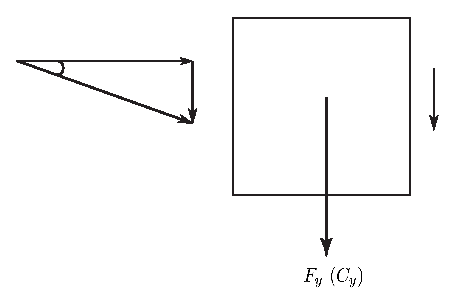
\includegraphics[width=0.5\unitlength]{../FnP/gnuplot/setup-1.eps}}         
      
      
   
 	\put(0.315,0.93){$U$}
 	\put(0.3,0.84){$U_i$}
    \put(0.42,0.88){$\dot{y}$}
    \put(0.28,0.895){ $\theta$}
    \put(0.7,0.87){\small $(+)$}
      	

 	
 	 

     

  \end{picture}

 \caption{Induced angle of attack on the square prism due to the resultant of free-stream velocity of the fluid and transverse velocity of the body.}
    \label{fig:setup_1}
\end{figure}

 Figure \ref{fig:induced_lift_sketch}  illustrates the motion of the body at a given instantaneous time.The induced angle of attack is formed on the square cross section as a result of the fressrteam velocity vector $U$ and the transverse velocity vector of the body $\dot{y}$. Thus, a force is formed in phase with the motion of the body (square cross section). This mechanism could also be observed on other bodies which are prone to galloping. The sign convention in this figure (and generally used in this scope of research) states that downward direction is positive. Hence, the force generated on a body under the influence of galloping, could be also identified as a ``negative lift".
 

\subsection{Quasi-steady state theory}
\label{sec:QSS theory}


According \cite{Paidoussis2010},the initial studies by \cite{Glauert1919} provided a criterion for galloping by considering the auto-rotation of a stalled aerofoil. As this phenomenon commonly occur in iced transmission lines, \cite{DenHartog1956} has provided a theoretical explanation for iced electric transmission lines. 

The pioneering study in order to mathematically model galloping was conducted by \cite{Parkinson1964}. This model has been widely used in almost all subsequent studies regarding galloping. A weakly non-linear oscillator model was developed by them to predict the response of the system. Essentially the quasi-steady assumption was made to develop this theory assuming that the instantaneous induced lift force of the oscillating body is equal to that of the lift force generated by the same body at the same induced angle of attack. In order to satisfy the quasi-steady assumption few conditions had to be satisfied.

\begin{itemize}
 \item The velocity of the body does not change rapidly
 \item There is no interaction between vortex shedding and galloping
\end{itemize}

The second condition is satisfied by ensuring the vortex shedding frequency is much higher than the galloping frequency.
The oscillator equation was solved using the Krylov and Bogoliubov method. Details of this method would not be mentioned as it is not used in the present study to solve the oscillator equation. The results obtained form experiments, carried out at $\reynoldsnumber=2200$ and a mass ratio (\mstar) around 1164 had a good agreement with the theoretical data which is shown in figure \ref{fig:parkinson_paper_data}.

\begin{figure}
	
  \setlength{\unitlength}{\textwidth}

        \begin{picture}(1,0.82)(0,0.4)

      % % % Parkinson Data 

      \put(0.05,0.39){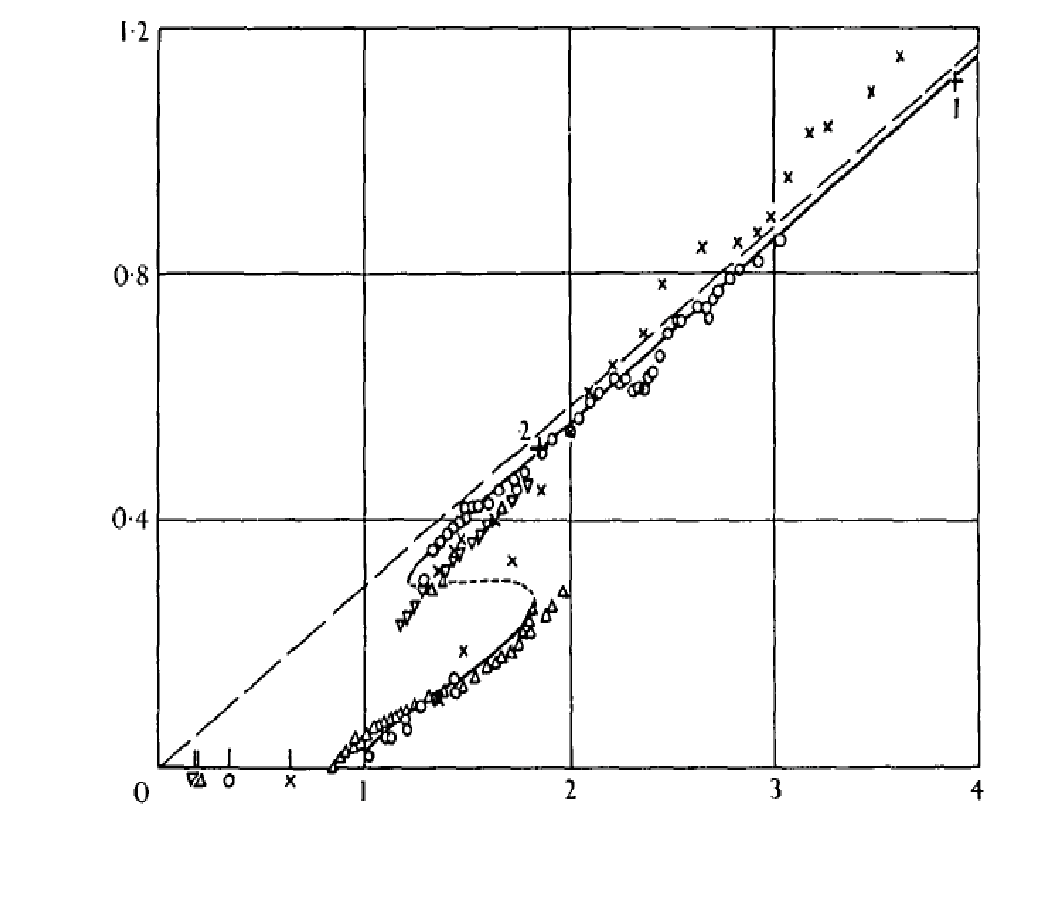
\includegraphics[width=0.9\unitlength]{./chapter-literature-revirw/fnp/parkinson_data.eps}}
      
%       \put(0.07,0.95){$\displaystyle\frac{V}{D}$}
%       \put(0.07,1.3){$\displaystyle\frac{A}{D}$}
       \put(0.05,0.8){\Large$\frac{nA}{2\beta}\bar{Y}_s$}
       \put(0.52,0.42){\Large$\frac{nA}{2\beta}U$}
       \
%\put(0.189,1.415){\small(a)}
%\put(0.189,1.07){\small(b)}
%\put(0.189,0.73){\small(c)}

%  


    \end{picture}

  \caption{``Collapsed amplitude-velocity characteristic. Theory: \solidrule \ stable limit cycle, \dashedrule unstable limit cycle. Experiment $\times \ \beta = .00107$, $\circ \ \beta =.00196$,\ $\vartriangle \beta=.00364$,$\triangledown \ \beta = .00372$,\ $+1 \ \beta=.0012$,\ $+2 \ \beta=.0032$ Reynolds numbers $4,000-20,000$ ". Figure extracted from \cite{Parkinson1964}. $\frac{nA}{2\beta}\bar{Y}_s$ is the dimensionless displacement amplitude parameter and $\frac{nA}{2\beta}U$ is the reduced velocity.$\beta$ is the damping ratio and $n=\frac{1}{\mstar}$. The experimental data shows a good agreement with the theoretical model.}
    \label{fig:parkinson_paper_data}
\end{figure}

 %vspace{10cm}


\subsubsection*{Quasi-steady state oscillator model}

The equation of motion of transversely oscillating body is given by 
\begin{equation}
\label{equationofmotion}
m\ddot{y}+c\dot{y}+ky=F_y,
\end{equation}
where the forcing term $F_y$ is given by
\begin{equation}
\label{lift equation}
F_y=\frac{1}{2}\rho U^2\mathcal{A}C_y.
\end{equation}

As explained previously, when quasi-steady assumption is used the stationary $C_y$ data (which consists of both lift and drag data)  of the body could be could be used as inputs to the oscillator equation.\citet{Parkinson1964} used a $7^th$ order odd interpolating polynomial to determine $C_y$. The order of the polynomial can be chosen arbitrarily depending on the study. For example \citet{Barrero-Gil2009,Barrero-Gil2010a} have used a $3_{rd}$ order polynomial in order to simplify the analytical model. However, \citet{Ng2005} pointed out that a $7_{th}$ order polynomial is sufficient as it does not provide a significantly better result.    

\begin{equation}
\label{cy ploynomial}
C_y(\theta)=a_1\left(\frac{\dot{y}}{U}\right)-a_3\left(\frac{\dot{y}}{U}\right)^3+a_5\left(\frac{\dot{y}}{U}\right)^5-a_7\left(\frac{\dot{y}}{U}\right)^7.
\end{equation}

Therefore by substituting the forcing function to the oscillator equation (Eq:\ref{equationofmotion}) the Quasi-steady state (QSS) model could be obtained (Eq:\ref{final_equation_motion}). 

\begin{equation}
\label{final_equation_motion}
m\ddot{y}{+}c\dot{y}{+}ky{=}\frac{1}{2}\rho U^2 \mathcal {A} \Bigg(a_1\left(\frac{\dot{y}}{U}\right){-}a_3\left(\frac{\dot{y}}{U}\right)^3{+}a_5\left(\frac{\dot{y}}{U}\right)^5{-}a_7\left(\frac{\dot{y}}{U}\right)^7 \Bigg).
\end{equation}

As the current study is focused on the low \reynoldsnumber region, it is a known fact that the vortex shedding will be correlated well and therefore provide a significant forcing in the low Reynolds number region. \citet{Joly2012} introduced and additional sinusoidal forcing function to the model in order to integrate the forcing by vortex shedding. By the addition of this forcing \citet{Joly2012} managed to obtain accurate predictions of the displacement amplitude even at low mass ratios, where the galloping is suppressed or not present. Yet, the strength or the amplitude of this sinusoidal forcing has to be tuned in an \emph{ad hoc} manner, and it was not clear the relationship between this forcing with the other system parameters. Thus in the current study this forcing was not used.

\subsubsection*{Presence of hysteresis}

Hysteresis could be observed in the in the amplitude data of \cite{Parkinson1964}. In contrast, the studies carried out by \citet{Barrero-Gil2009} and \citet{Joly2012} at much lower Reynolds numbers ($159\leq \reynoldsnumber\leq 200$), did not show any hysteresis. \citet{Luo2003} concluded that the hysteresis was present due to the presence of an inflection point in the $C_y$ curve at high Reynolds numbers (\citet{Parkinson1964} data) which was not present at lower Reynolds numbers. It was further explained and demonstrated by Luo that the inflection point occurs due to the intermittent re attachment of the shear layer in certain angles at high Reynolds numbers. 

% % % consider putting luos data % % % % % %  


% % solving method  ???


\subsection{Induced force and the shear layers}
\label{subsec:c_y and shear layers}

It is important to have an understanding on how the induced lift is generated in a fluid dynamics point of view. The quasi-steady model has already been validated and re-validated by many studies, therefore the flow-field data of static body simulations could be used to analyse the underpinning fluid dynamic mechanisms governing galloping.

\begin{figure}[t!]

  \setlength{\unitlength}{\textwidth}

  \begin{picture}(1,0.35)(0,0.725)

    \put(-0.01,0.76){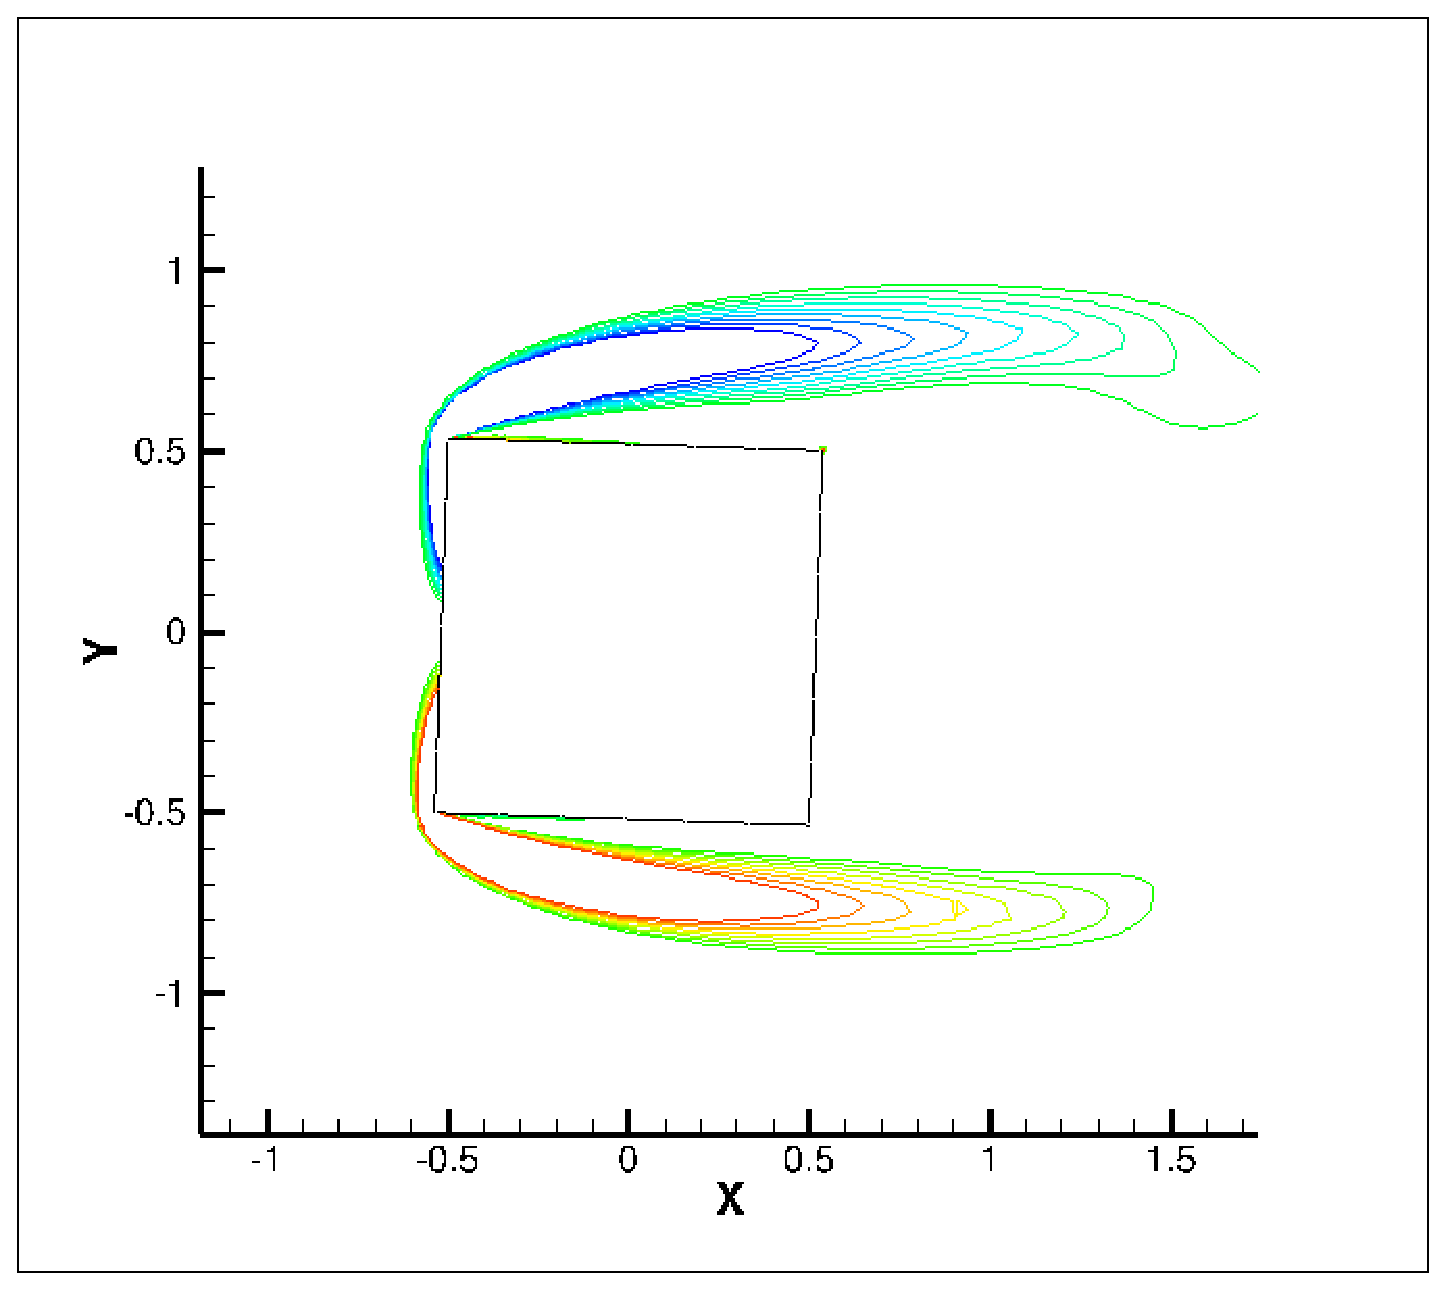
\includegraphics[width=0.33\unitlength]{./chapter-literature-revirw/fnp/square-2.eps}}
    \put(0.335,0.76){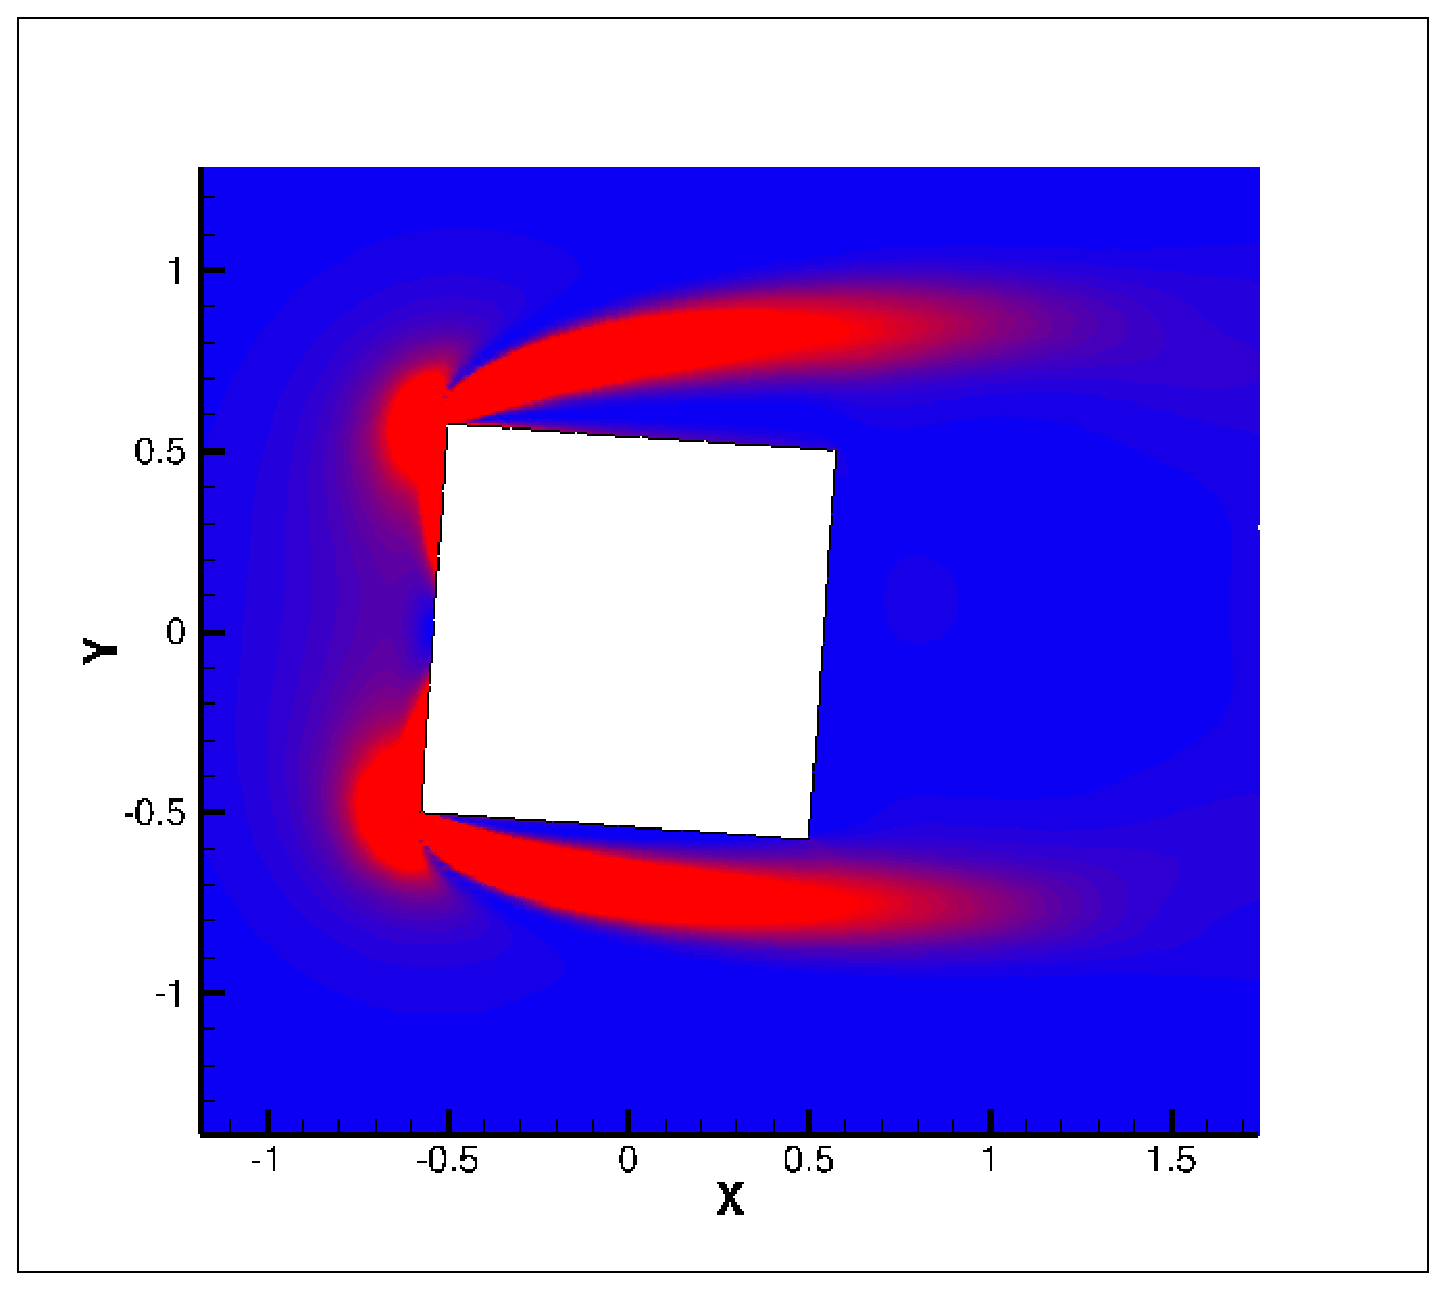
\includegraphics[width=0.33\unitlength]{./chapter-literature-revirw/fnp/square-4.eps}}
    \put(0.68,0.76){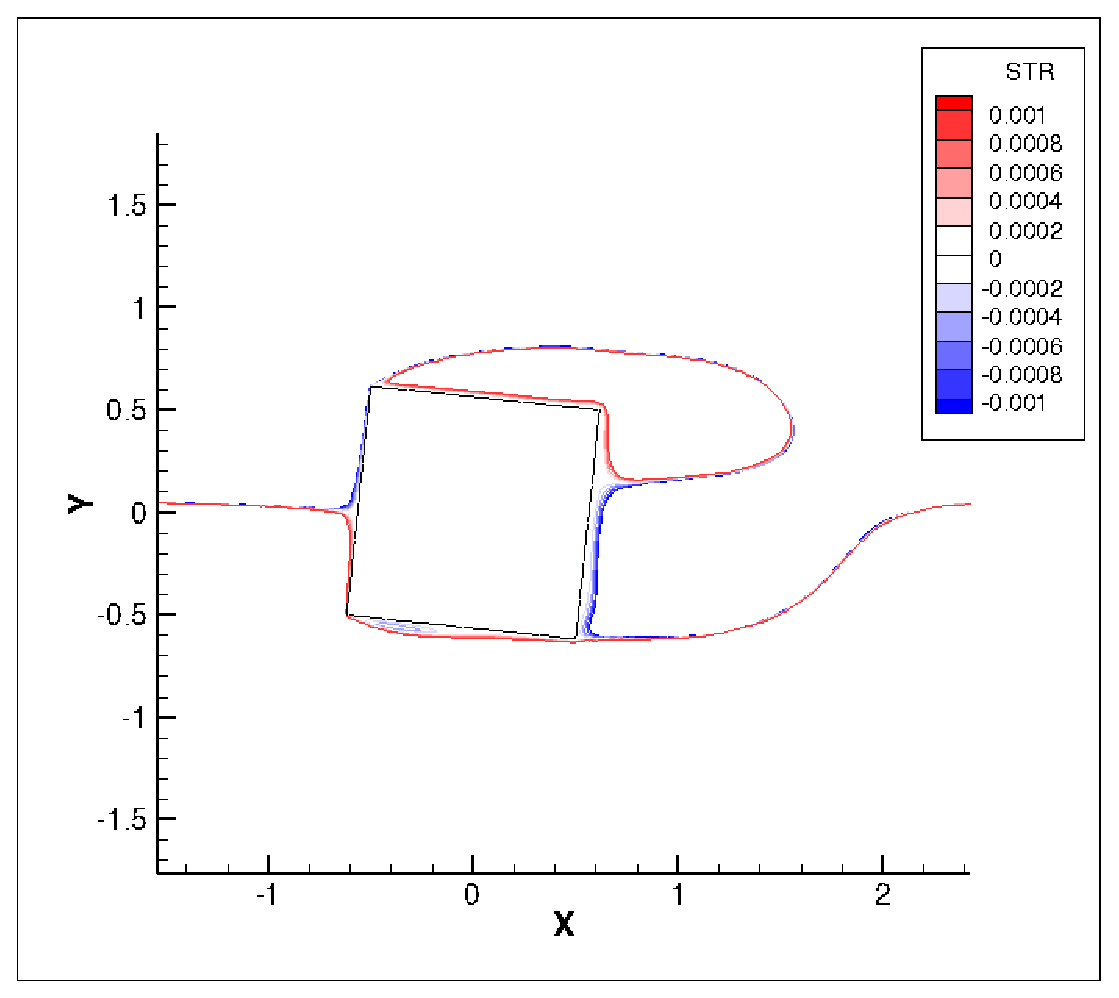
\includegraphics[width=0.33\unitlength]{.//chapter-literature-revirw/fnp/square-6.eps}}

   
    
    \put(0.0,0.735){(a)}    
    \put(0.34,0.735){(b)}
    \put(0.685,0.735){(c)}
  
  \end{picture}

  \caption{Stream functions of time averaged flow field on a stationary square section at $\reynoldsnumber=200$ at different incidence angles. (a) $2^{\circ}$ ($C_{y}$ increases),(b) $4^{\circ}$ ($C_{y}$ peaks) and (c) $2^{\circ}$ ($C_{y}$ decreases). The bottom shear layer comes closer to the bottom wall and reattaches as the angle of incidence increases.}
  \label{fig:shear_layers}
\end{figure}






The governing mechanism of galloping is the behaviour of the shear layers created at the leading edge due to flow separation  on the top and bottom of the body. A common example is a square cross section which has been used widely in studies on galloping. In this square cross section (figure \ref{fig:shear_layers}) the flow separate from the leading edges of the body and create two shear layers on the top and bottom sides of the the body. Figure \ref{fig:shear_layers} shows the stream functions of time averaged (over a vortex shedding cycle) flow fields of stationary cross sections. The angle of incidence increases clockwise from $2^{\circ}-6^{\circ}$. As $\theta$ is increased, the bottom shear comes closer to the wall of the body compared to the top shear layer (Figure \ref{fig:shear_layers} (a)). The shear layer nearer to the body crates higher suction compared to the shear layer at the opposite side. This pressure imbalance between the top and bottom sides of the body creates a downward force (i.e. the negative lift). As the angle is increased, the bottom shear layer becomes more closer and therefore the pressure difference becomes grater leading to a higher $C_{y}$. The negative lift force becomes maximum when the shear layer near to the wall reattaches at the trailing edge (figure \ref{fig:shear_layers} (b)). As $\theta$ is further increased, the bubble in the bottom shear layer shrinks in size resulting the reduction of the pressure imbalance of the top and bottom surface leading to the reduction in $C_{y}$. \hilight{put the cY curve as crodd reference}. As the body is connected to an oscillatory system (discussed in section \ref{sec:exci-galloping}), this shear layer behaviour also harmonize with the cyclic behaviour of the system providing the driving force to the system so that the motion of galloping is sustained.



\subsection{Frequency response}
 
 It is clear that the cyclic motion of the shear layer harmonize with the mechanical system. Therefore, the frequency response should be then, the natural frequency of the system $\omega_{n}$ which much is different from VIV mechanism, where the primary frequency comes from the periodic forcing of the vortex shedding. Hence, in the QSS model the natural frequency of the system could be identified as the frequency of oscillations. However, it should be  noted that this is valid on the regimes where the conditions discussed in section \ref{sec:QSS theory} are satisfied. 
 
 On the other hand, the forcing function in the QSS model equation \ref{final_equation_motion}, is a non linear function. As the mass ratio is quite high, the non-linearities of the forcing does not make much effect to the frequency response. However, as the mass ratio goes down theoretically the non linearities of the forcing should affect the frequency response of the system.   
 
 The experimental studies carried by \citet{bouclin:77} concluded at high reduced velocities with large inertia, the motion of the cylinder controls the frequency of the system rather than the vortex shedding. The structural damping has no effect provided that it is small. He also concluded that as the inertia and the reduced velocity gets lower, there is some interaction between vortex shedding and galloping. And at this region the frequency is mainly governed by the vortex shedding. 
 
 
 \subsection{Fluid mechanics governing the galloping response}
 
 As discussed in subsection \ref{subsec:c_y and shear layers} the driving force of a galloping system is the asymmetrical placement of the shear layers at either sides of the body. In consequence, it is clear that a significant afterbody is needed for the shear layer interaction to sustain galloping. \citet{Parkinson1974,Parkinson1989} and \citet{Bearman1987} have discussed well the importance of the length and the shape for galling in their reviews. It is also highlighted in \citet{Parkinson1974} that the most important physical parameters for galloping are the size relative to the characteristic hight and the shape of the afterbody. Manipulating the shape of the afterbody and thereby, manipulating the shear layer interactions with the body, gives the ability to control the galloping response. Thus, due to this reason work has been carried out on the response of galloping of different cross sectional shapes. 
 
 \citet{Blevins1990} provided a good comparison of the shapes which are prone to galloping based on the work by \citet{Parkinson1961}, \citet{Nakamura1975a} and \citet{Nakamura1977}. The reproduction of Blevins's data could be found in \citet{Paidoussis2010} presented in figure \ref{fig:par_diff_cross_sec}. 
    
 \begin{figure}
	
  \setlength{\unitlength}{\textwidth}

\fbox{
        \begin{picture}(1,1.2)(0,0.5)

      % % % Parkinson Data 

      \put(0.05,0.52){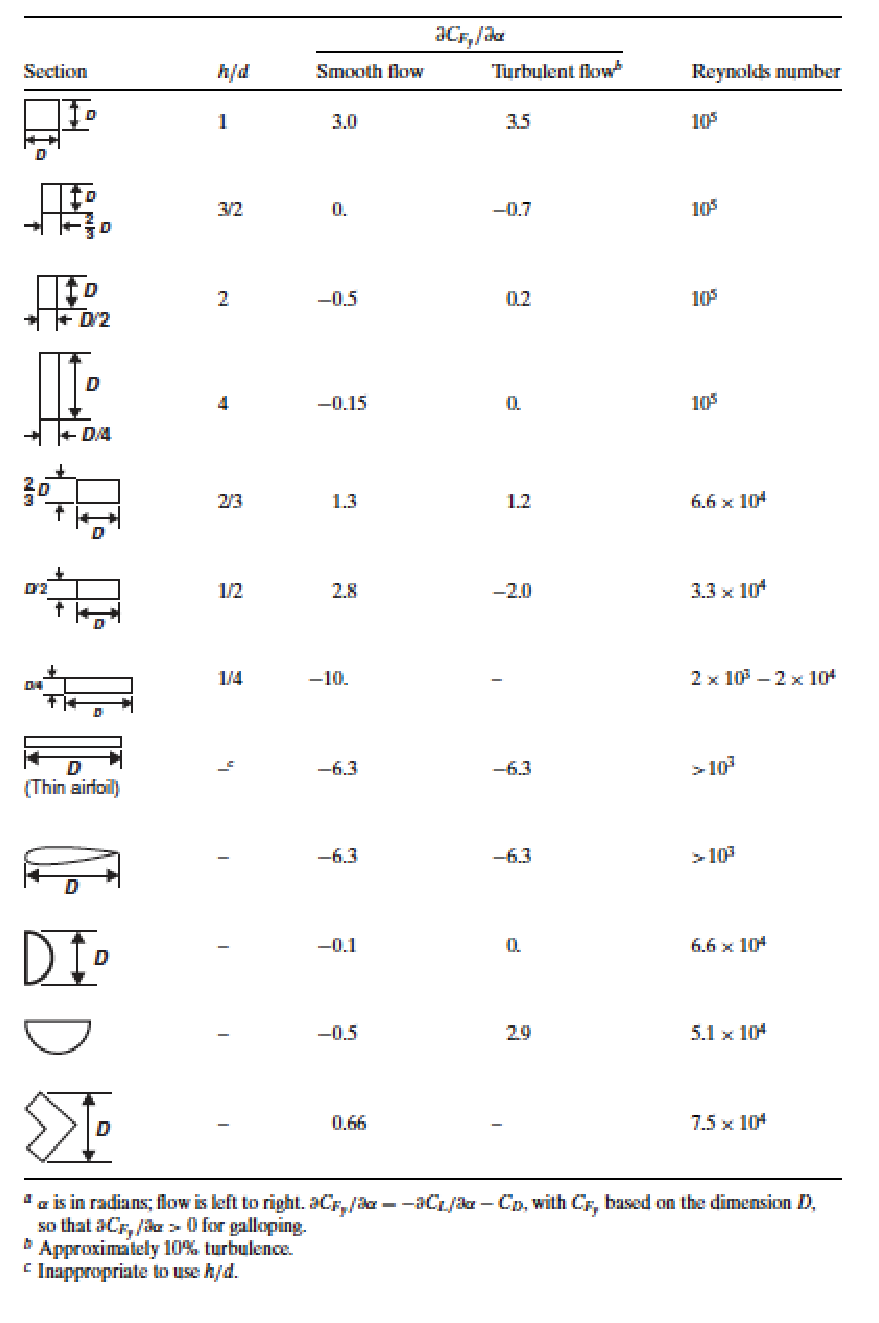
\includegraphics[width=0.75\unitlength]{./chapter-literature-revirw/fnp/per_cross_sec.eps}}
        


    \end{picture}
}
  \caption{ ``The transverse force coefficient for various sections in steady smooth or turbulent flow (after \citet{Blevins1990})" obtained from \citet{Paidoussis2010}. Here the induced angle is represented by $\alpha$ and the transverse force force coefficient is represented by $C_{fy}$. In order for galloping to sustain, the direction of both of these quantities should be same and thus have to satisfy the condition of $\frac{\partial C_{fy}}{\partial \alpha } >0$.}
    \label{fig:par_diff_cross_sec}
\end{figure}

 %vspace{10cm}

  
  
  \citet{Naudascher1993}, \citet{Ruscheweyh1996}, \citet{Deniz1997} and \citet{Weaver2005} are some of the work done on different cross sectional shapes.
 
 

 
 
 
 

 
 
 
 
 
 
 
 























  


    

     










